\documentclass{report}

% packages -> http://www.howtotex.com/packages/9-essential-latex-packages-everyone-should-use/
\usepackage[utf8]{inputenc}
\usepackage{hyperref}
\usepackage{amsmath,amssymb,amsthm,amsfonts,mathtools,mathrsfs}
\usepackage{tocbibind}
\usepackage{bbm}
\usepackage{enumitem}
\usepackage{fancyhdr}			% per i numeri di pagina
\usepackage[a4paper,margin=0.8in]{geometry}	% to adjust the margins of pages
\usepackage{graphicx}			% for inserting figures
\usepackage{microtype}			% document reads better
% \usepackage[backend=bibtex,style=numeric]{biblatex}
\usepackage[toc]{appendix}
\usepackage{todonotes}
\usepackage{geometry}
\usepackage{subfigure}
\usepackage{algorithm}
\usepackage[noend]{algpseudocode}
\usepackage{listings}
\usepackage{color}
\usepackage{caption}

\newcommand{\inputfrom}[1]{\input{./tex/#1/#1}}

\setcounter{MaxMatrixCols}{30}
\providecommand{\U}[1]{\protect\rule{.1in}{.1in}}
\newtheorem{theorem}{Theorem}
\newtheorem{acknowledgement}[theorem]{Acknowledgement}
\newtheorem{axiom}[theorem]{Axiom}
\newtheorem{case}[theorem]{Case}
\newtheorem{claim}[theorem]{Claim}
\newtheorem{conclusion}[theorem]{Conclusion}
\newtheorem{condition}[theorem]{Condition}
\newtheorem{conjecture}[theorem]{Conjecture}
\newtheorem{corollary}[theorem]{Corollary}
\newtheorem{criterion}[theorem]{Criterion}
\newtheorem{definition}[theorem]{Definition}
\newtheorem{example}[theorem]{Example}
\newtheorem{exercise}[theorem]{Exercise}
\newtheorem{lemma}[theorem]{Lemma}
\newtheorem{notation}[theorem]{Notation}
\newtheorem{problem}[theorem]{Problem}
\newtheorem{proposition}[theorem]{Proposition}
\newtheorem{remark}[theorem]{Remark}
\newtheorem{solution}[theorem]{Solution}
\newtheorem{summary}[theorem]{Summary}

\graphicspath{ {img/} }

\DeclarePairedDelimiter\ceil{\lceil}{\rceil}
\DeclarePairedDelimiter\floor{\lfloor}{\rfloor}

\renewcommand*\thelstnumber{\arabic{lstnumber}:}

\DeclareCaptionFormat{mylst}{\hrule#1#2#3}
\captionsetup[lstlisting]{format=mylst,labelfont=bf,singlelinecheck=off,labelsep=space}

\definecolor{mygreen}{rgb}{0,0.6,0}
\definecolor{mygray}{rgb}{0.5,0.5,0.5}
\definecolor{mymauve}{rgb}{0.58,0,0.82}

\lstset{ %
  backgroundcolor=\color{white},   % choose the background color; you must add \usepackage{color} or \usepackage{xcolor}; should come as last argument
  basicstyle=\footnotesize,        % the size of the fonts that are used for the code
  breakatwhitespace=false,         % sets if automatic breaks should only happen at whitespace
  breaklines=true,                 % sets automatic line breaking
  captionpos=b,                    % sets the caption-position to bottom
  commentstyle=\color{mygreen},    % comment style
  deletekeywords={...},            % if you want to delete keywords from the given language
  escapeinside={\%*}{*)},          % if you want to add LaTeX within your code
  extendedchars=true,              % lets you use non-ASCII characters; for 8-bits encodings only, does not work with UTF-8
  frame=single,	                   % adds a frame around the code
  keepspaces=true,                 % keeps spaces in text, useful for keeping indentation of code (possibly needs columns=flexible)
  keywordstyle=\color{blue},       % keyword style
  language=C,              		   % the language of the code
  morekeywords={*,...},            % if you want to add more keywords to the set
  numbers=left,                    % where to put the line-numbers; possible values are (none, left, right)
  numbersep=5pt,                   % how far the line-numbers are from the code
  numberstyle=\tiny\color{mygray}, % the style that is used for the line-numbers
  rulecolor=\color{black},         % if not set, the frame-color may be changed on line-breaks within not-black text (e.g. comments (green here))
  showspaces=false,                % show spaces everywhere adding particular underscores; it overrides 'showstringspaces'
  showstringspaces=false,          % underline spaces within strings only
  showtabs=false,                  % show tabs within strings adding particular underscores
  stepnumber=2,                    % the step between two line-numbers. If it's 1, each line will be numbered
  stringstyle=\color{mymauve},     % string literal style
  tabsize=2,	                   % sets default tabsize to 2 spaces
  title=\lstname                   % show the filename of files included with \lstinputlisting; also try caption instead of title
}

\hypersetup{
    backref,
    bookmarks=true,         % show bookmarks bar?
    unicode=false,          % non-Latin characters in Acrobat’s bookmarks
    pdftoolbar=true,        % show Acrobat’s toolbar?
    pdfmenubar=true,        % show Acrobat’s menu?
    pdffitwindow=false,     % window fit to page when opened
    pdfstartview={FitH},    % fits the width of the page to the window
    pdftitle={Network of interacting neurons with random synaptic weights},    % title
    pdfauthor={Grazieschi Paolo \& Leocata Marta \& Mascart Cyrille},     % author
    pdfsubject={Study of the mean-field equation of a network of interacting leacky integrate and fire neurons},   % subject of the document
    pdfcreator={Grazieschi Paolo \& Leocata Marta \& Mascart Cyrille},   % creator of the document
    pdfproducer={Grazieschi Paolo \& Leocata Marta \& Mascart Cyrille}, % producer of the document
    pdfkeywords={neurons, mean-field, fokker-planck, stochastic process}, % list of keywords
    pdfnewwindow=true,      % links in new PDF window
    colorlinks=true,       % false: boxed links; true: colored links
    linkcolor=red,          % color of internal links (change box color with linkbordercolor)
    linkbordercolor=white,
    citecolor=green,        % color of links to bibliography
    filecolor=magenta,      % color of file links
    urlcolor=cyan,           % color of external links
    urlbordercolor=white
}

\captionsetup{compatibility=false}
\DeclareCaptionSubType*{algorithm}
\renewcommand\thesubalgorithm{\thetable\alph{subalgorithm}}
\DeclareCaptionLabelFormat{alglabel}{Alg.~#2}

\algnewcommand\algorithmicto{\textbf{to}}
\algrenewtext{For}[3]{%
  \algorithmicfor\ #1 $\gets$ #2 \algorithmicto\ #3 \algorithmicdo
}
\algnewcommand\COMMENT[2][.1\linewidth]{%
  \leavevmode\hfill\makebox[#1][l]{$\triangleright$~#2}
}
\algnewcommand\RETURN{\State \textbf{return} }

\tikzstyle{vecArrow} = [thick, decoration={markings,mark=at position
   1 with {\arrow[semithick]{open triangle 60}}},
   double distance=1.4pt, shorten >= 5.5pt,
   preaction = {decorate},
   postaction = {draw,line width=1.4pt, white,shorten >= 4.5pt}]
\tikzstyle{innerWhite} = [semithick, white,line width=1.4pt, shorten >= 4.5pt]

\renewcommand{\d}[1]{\ensuremath{\operatorname{d}\!{#1}}}

\everymath{\displaystyle}

\begin{document}
	\begin{figure}
		\begin{subfigure}{\textwidth}
			\centering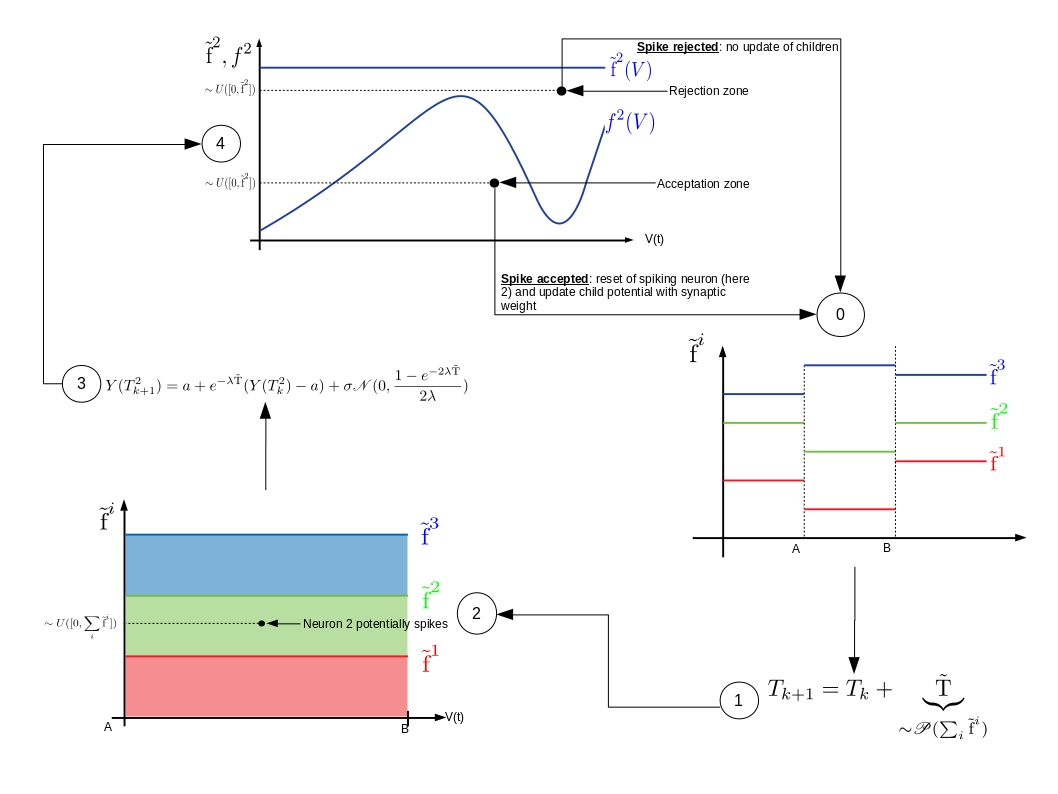
\includegraphics{rejectaccept}
		\end{subfigure}
		\begin{subalgorithm}{\textwidth}
			\caption{Pseudo code of the thinning algorithm used for simulating the system}
			\label{alg:pseudo-code}
			\centering\begin{algorithmic}
				\State Initialize all parameters
				\Repeat
					\Repeat\COMMENT{Steps 0-1}
						\State determine an interval $[t_{n-1},t_n]$ on which sampling
						\State compute the array of $f_{max}(Y_{t_{n-1}})$ and $\sum f_{max}(Y_{t_{n-1}})$ on interval $[t_{n-1},t_n]$
						\State $t_n\sim t_{n-1}+\mathscr{E}(\sum f_{max})$
					\Until{not in good interval or all $f_{max}$ are at 0}
					\State $u\sim\mathbb{U}([0,1])\rightarrow \mathbb{P}(\text{spiking neuron is neuron i})=\frac{f_{max}^i(Y_{t_n}^i)}{\sum_j^N f_{max}^j(Y_{t_n}^j)}$\COMMENT{Step 2}
					\State $u\sim\mathbb{U}([0,1])\rightarrow \mathbb{P}(\text{accepting spike of neuron i})=\frac{f^i(Y_{t_n}^i)}{f_{max}^i(Y_{t_n}^i)}$\COMMENT{Step 3}
					\If{ spike is accepted }\COMMENT{Step 4}
						update the potentials of all postsynaptic neurons
					\EndIf
				\Until{do not have the good amount of accepted spikes}
			\end{algorithmic}
		\end{subalgorithm}
		\label{fig:rejacc}
	\end{figure}
	The algorithm is presented in figure~\ref{fig:rejacc}. It explicits the several steps for simulating the network of neurons. The first step (0) is looking for a time interval, where the next event shall be looked for. The separation between two sequential events follow a Poisson distribution of parameter the sum of approximation function $T_{k+1}=T_k+\text{\~T}\text{, with }\mathscr{P}(\sum_i\text{\~f}^i)$.
	\begin{figure}
		\begin{subfigure}{\textwidth}
			\centering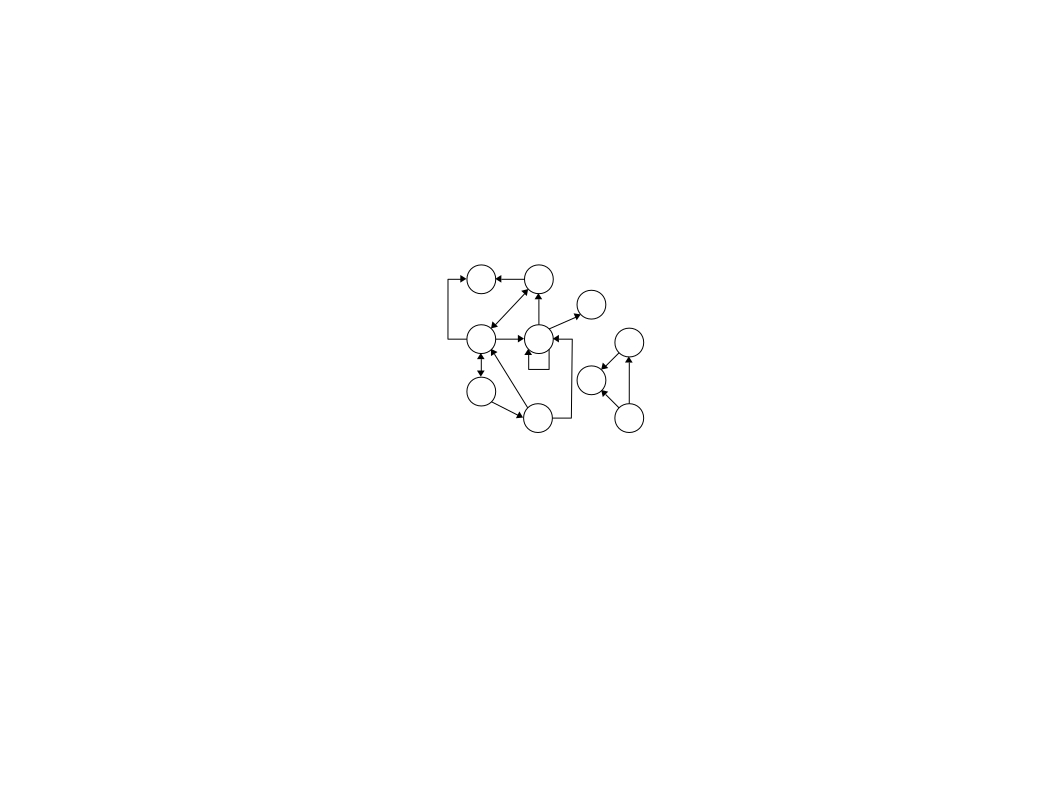
\includegraphics{complete_graph}
		\end{subfigure}
		\begin{subfigure}{\textwidth}
			\centering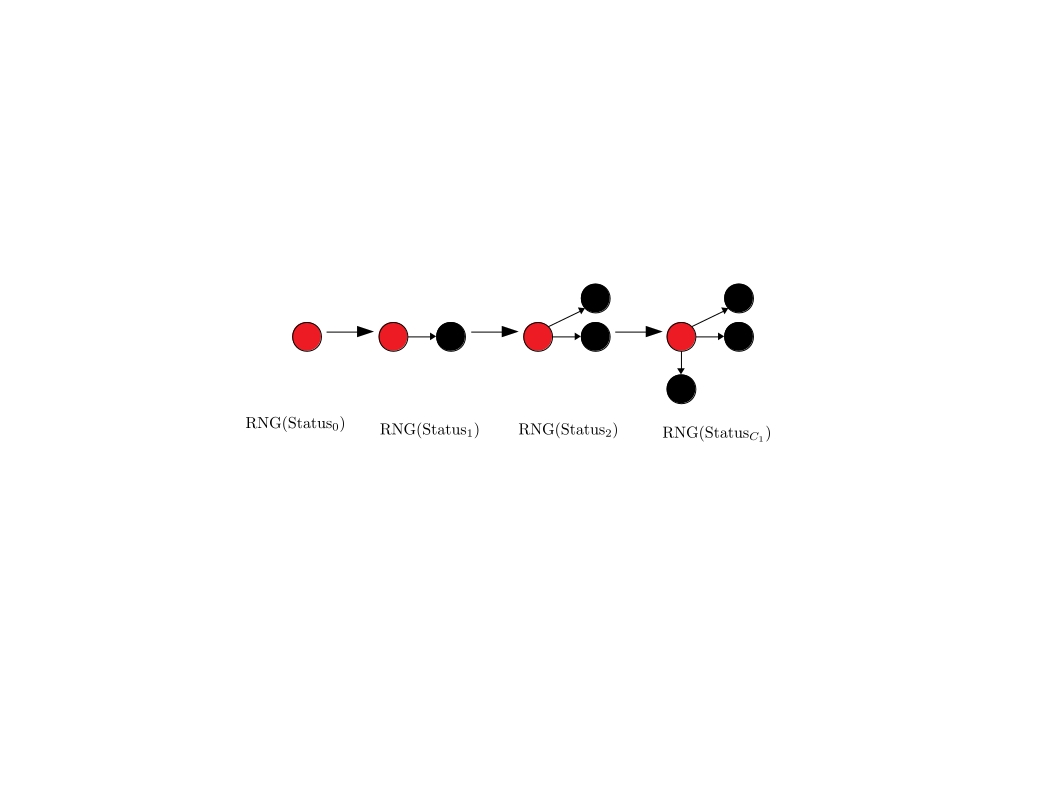
\includegraphics[width=.45\textwidth]{reconstruction1}
			\centering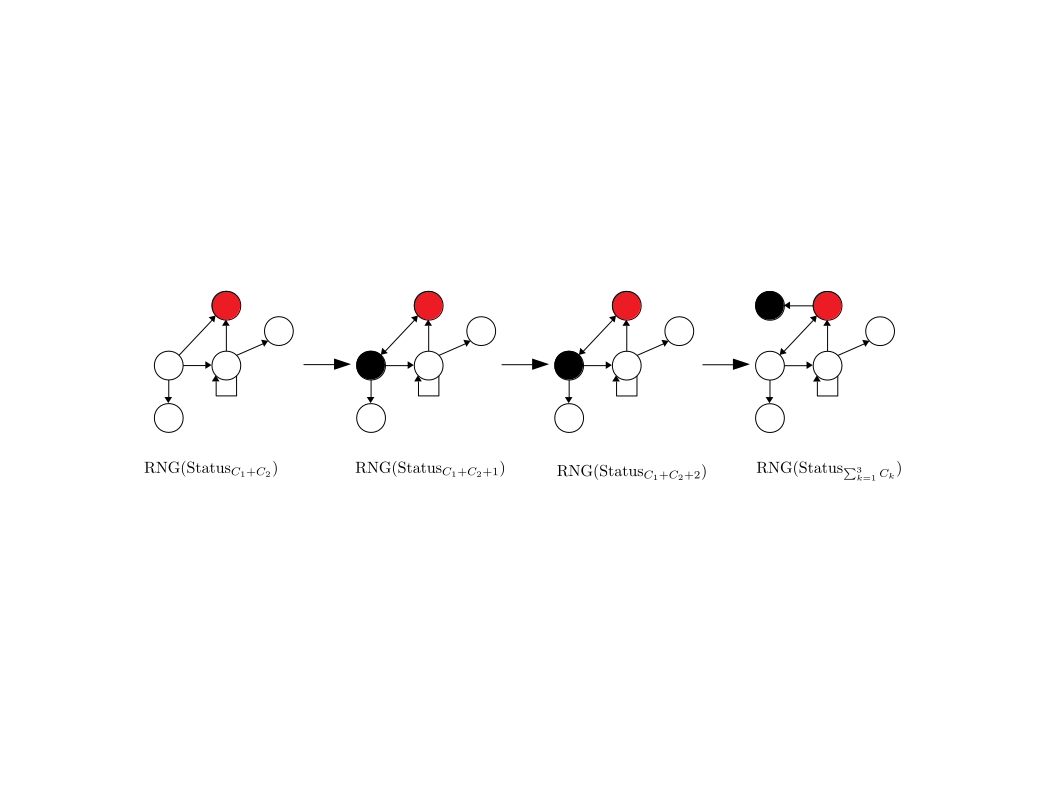
\includegraphics[width=.45\textwidth]{reconstruction2}\\
			\centering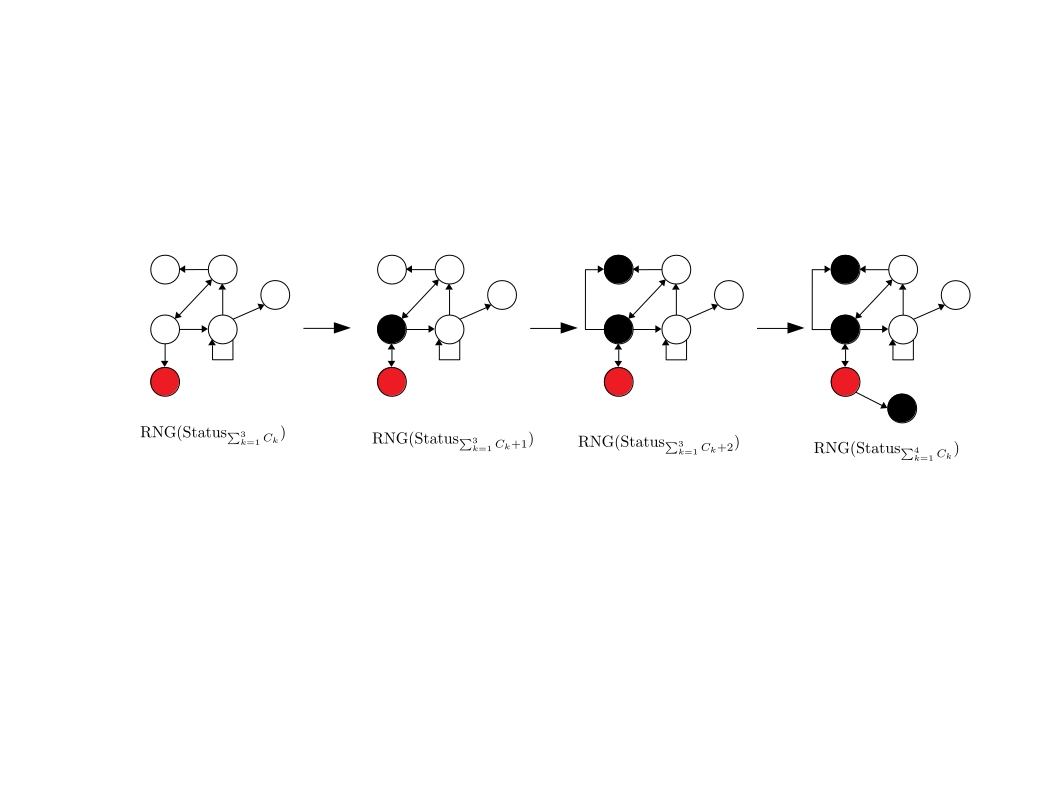
\includegraphics[width=.45\textwidth]{reconstruction3}
			\centering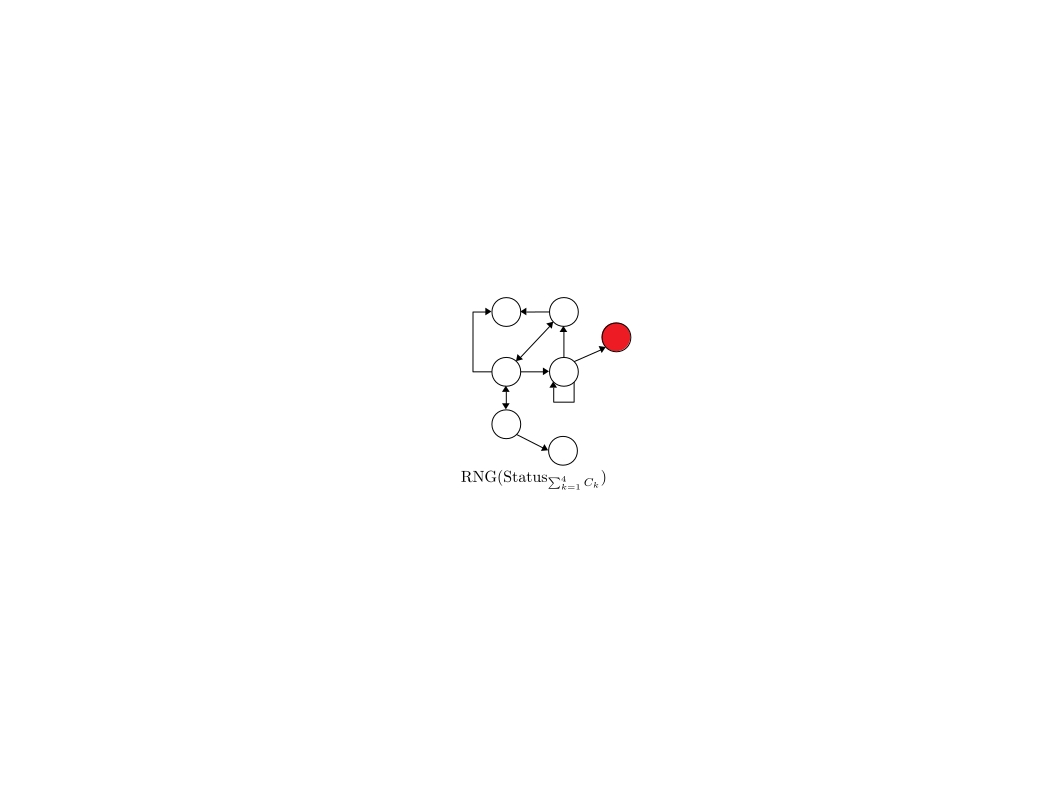
\includegraphics[width=.45\textwidth]{reconstruction4}\\
		\end{subfigure}
		\begin{subfigure}{\textwidth}
			\centering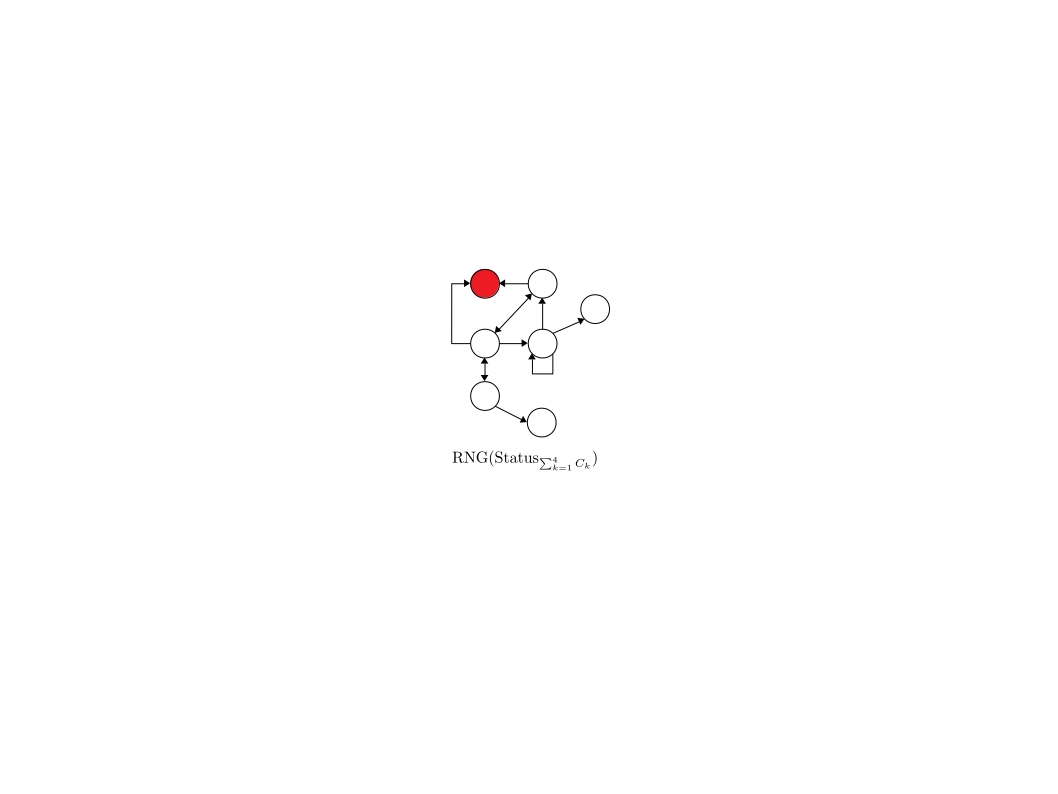
\includegraphics[width=.45\textwidth]{reconstruction5}
			\centering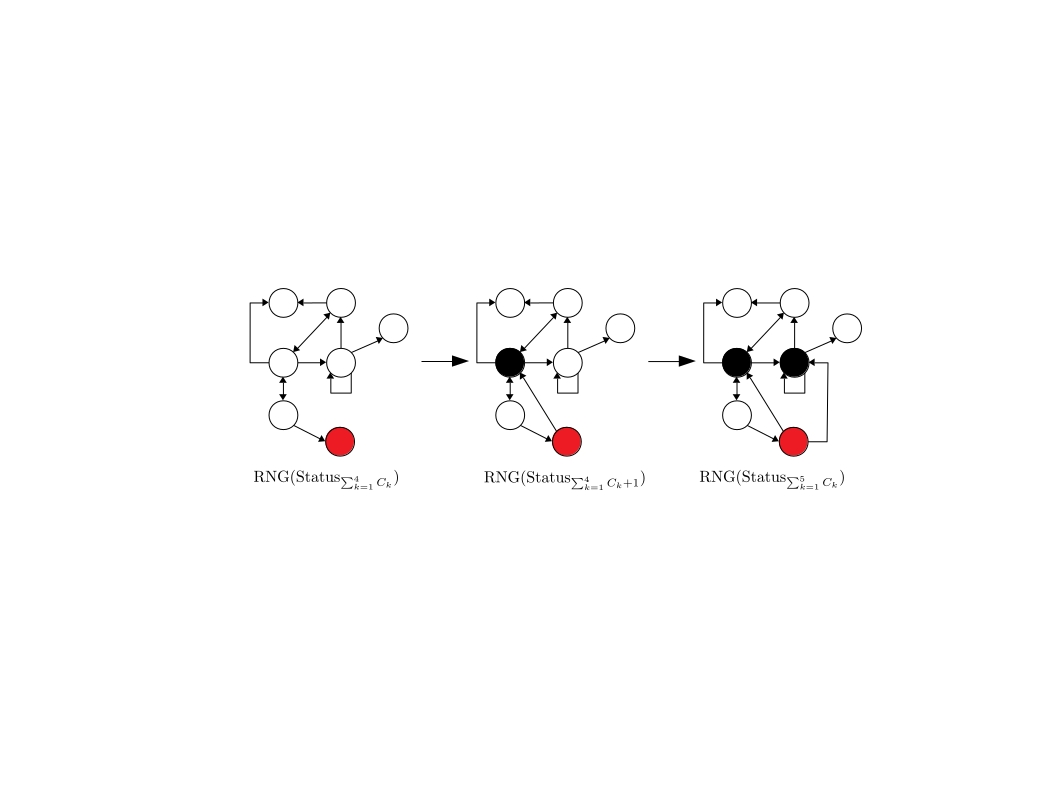
\includegraphics[width=.45\textwidth]{reconstruction6}\\
			\centering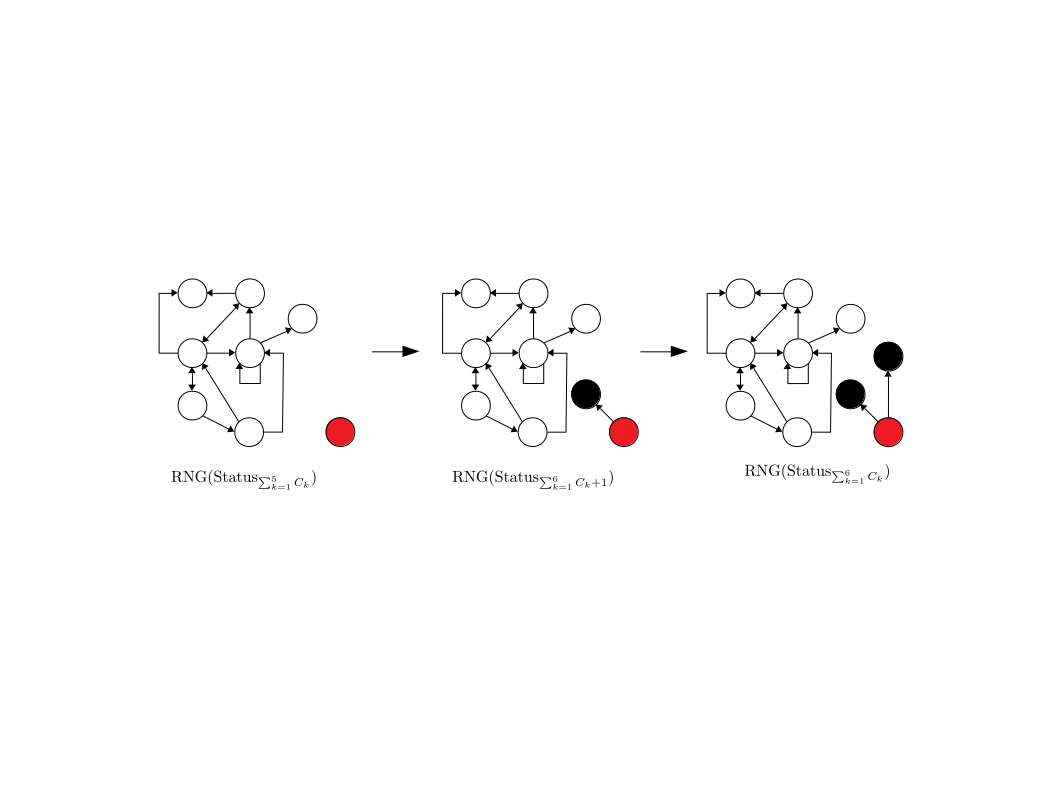
\includegraphics[width=.45\textwidth]{reconstruction7}
			\centering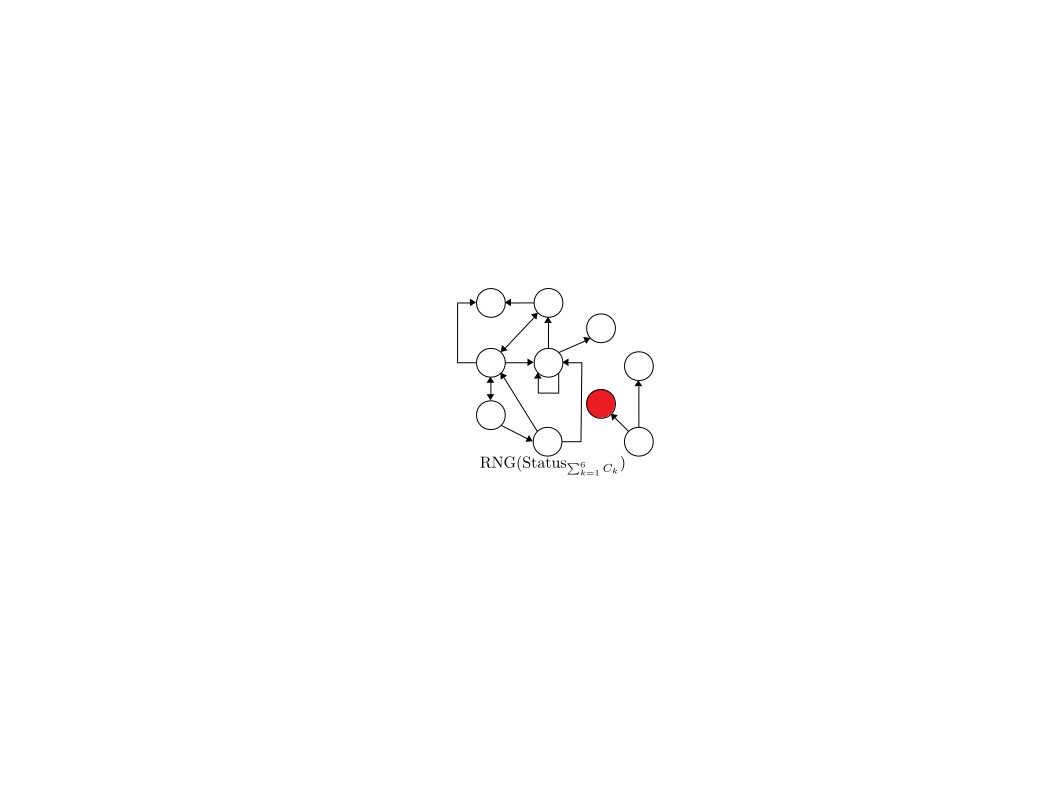
\includegraphics[width=.45\textwidth]{reconstruction8}\\
			\centering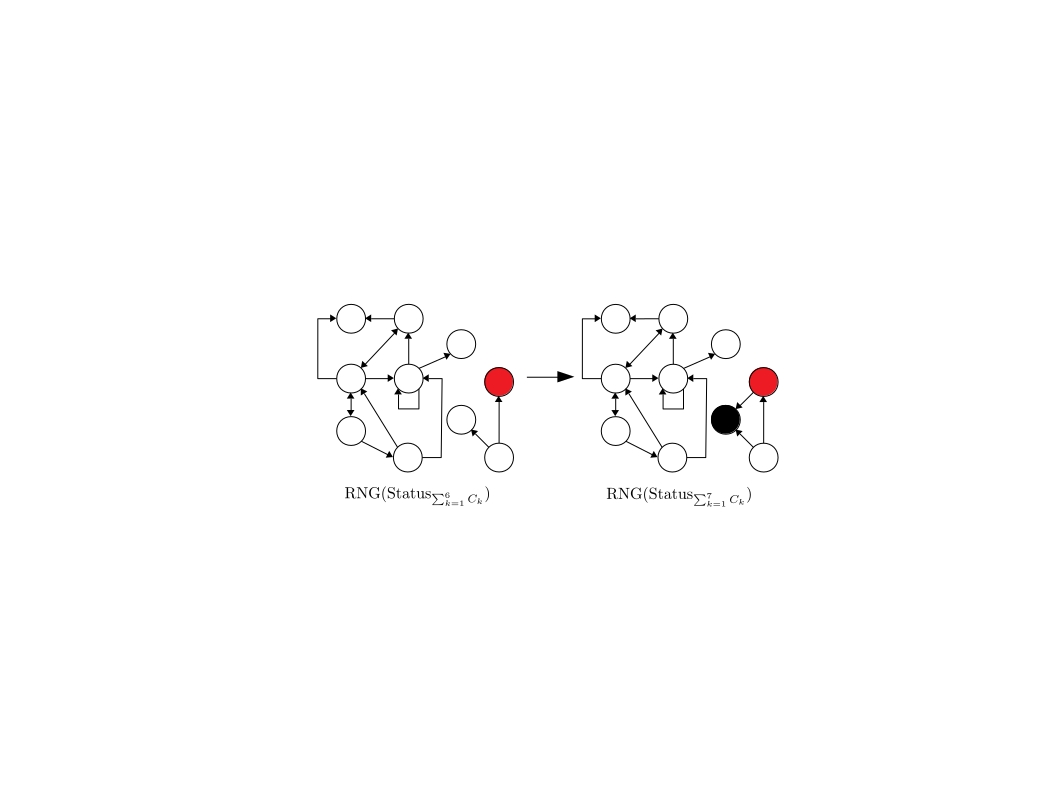
\includegraphics[width=.45\textwidth]{reconstruction9}
		\end{subfigure}
		\centering\begin{subalgorithm}{\textwidth}
			\begin{algorithmic}[1]
				\State RNG: a random number generator
				\State p: probability of connection between two neurons
				\State $\mathscr{M}_{i,j}$: matrix of interaction
				\Function{Interaction matrix}{RNG, p}
					\ForAll{$(i,j)\in\{1,\cdots,n\}^2$}
						\State $\mathscr{M}_{i,j}\gets\Call{RNG.B}{p}$
					\EndFor
				\EndFunction
			\end{algorithmic}
			\caption{Generation of a matrix of children}\label{alg:mat}
		\end{subalgorithm}\\
		\centering\begin{subalgorithm}{\textwidth}
			\begin{algorithmic}[1]
				\State RNG: a random number generator
				\State p: probability of connection between two neurons
				\State $V^s$: vector of states
				\State $V^c_i$: vector of children of neuron i
				\Function{Reconstructible}{RNG, p}
					\For{i}{1}{n}
						\State $V^s_i\gets$\Call{RNG.State}{}
						\For{j}{1}{n}
							\State \Call{RNG.B}{p}\COMMENT{Generate, \textbf{without storing them}, the children of i}
						\EndFor
					\EndFor
					\RETURN $V^s_i$
				\EndFunction
				\Function{Reconstruct}{RNG, i, $V^s$}
					\State \Call{RNG.setState}{$V^s$[i]}
					\For{j}{1}{n}
						\State $V^c_i[j]\gets$\Call{RNG.B}{p}
					\EndFor
					\RETURN $V^c_i$
				\EndFunction
			\end{algorithmic}
			\caption{Generation of a vector of rng states}\label{alg:vect}
		\end{subalgorithm}
	\end{figure}

	\begin{figure}
		\begin{subfigure}{\textwidth}
			\centering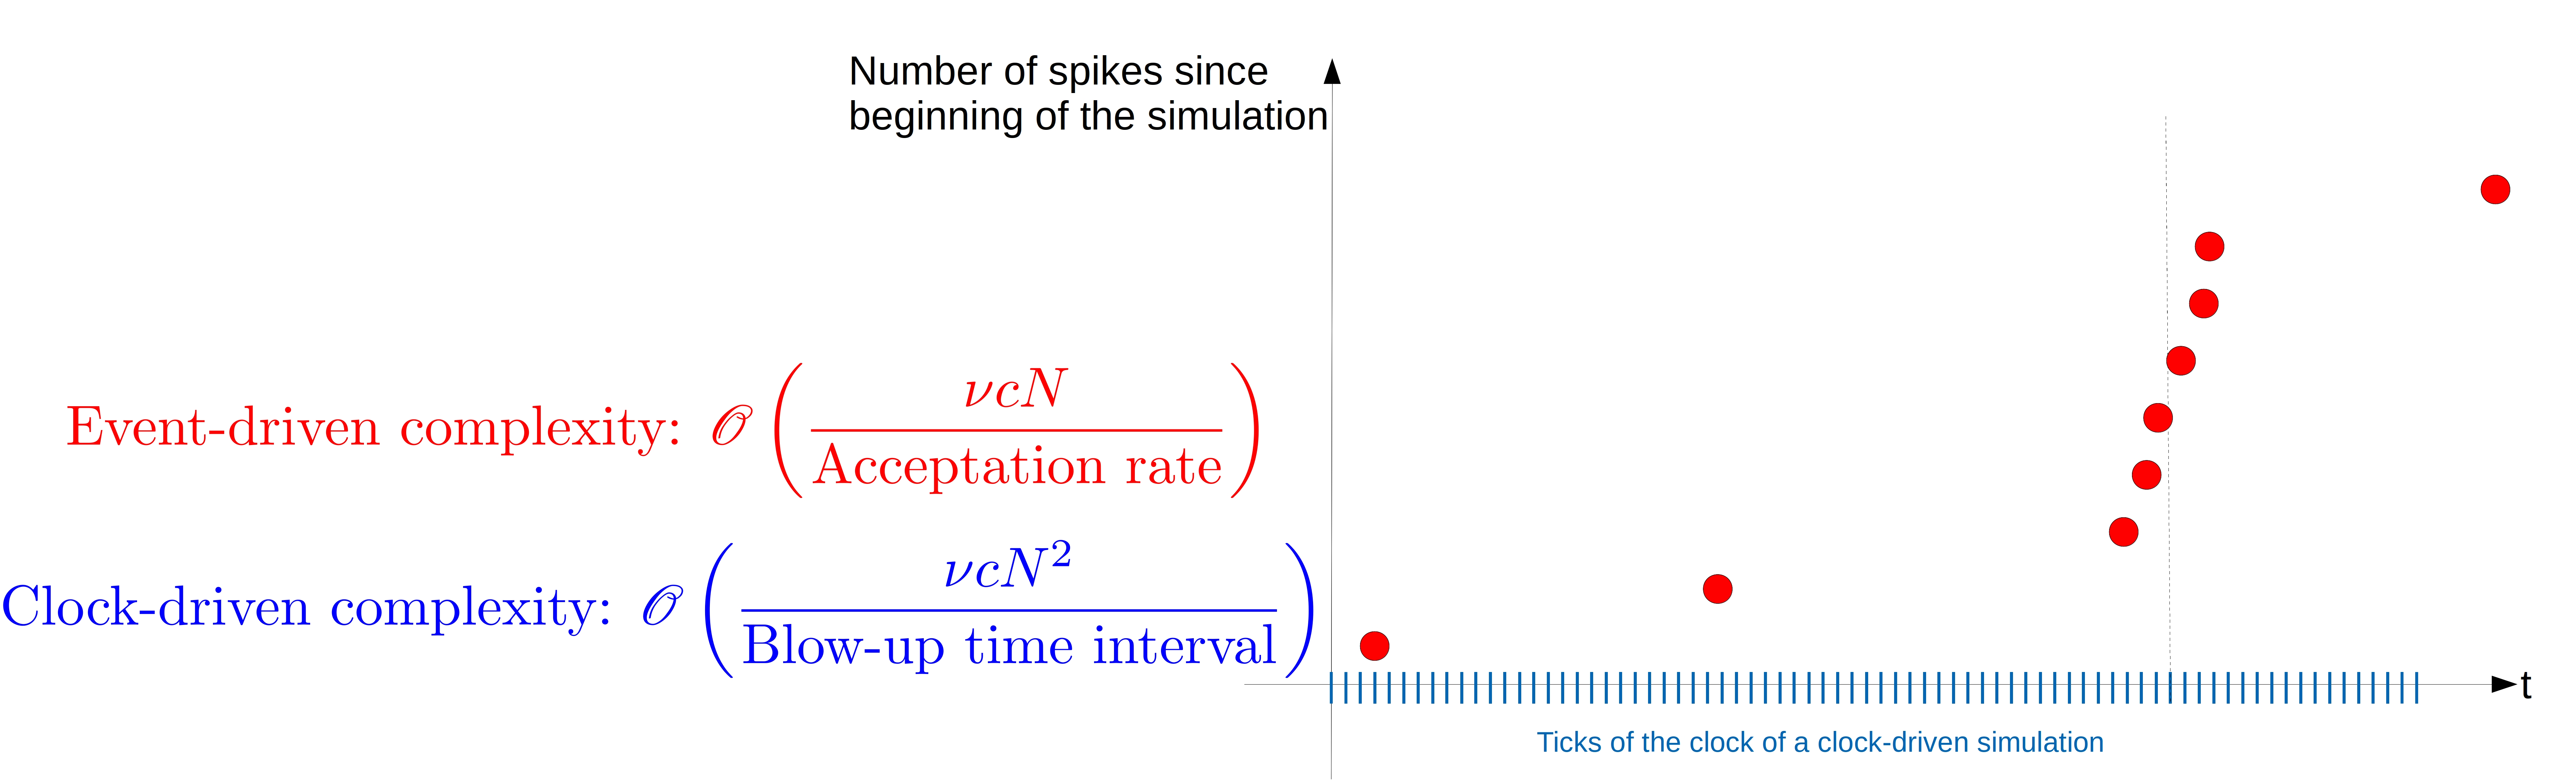
\includegraphics{complexity}
			\caption{Complexity as number of events during a time interval}
		\end{subfigure}
		\begin{subfigure}{\textwidth}
			\centering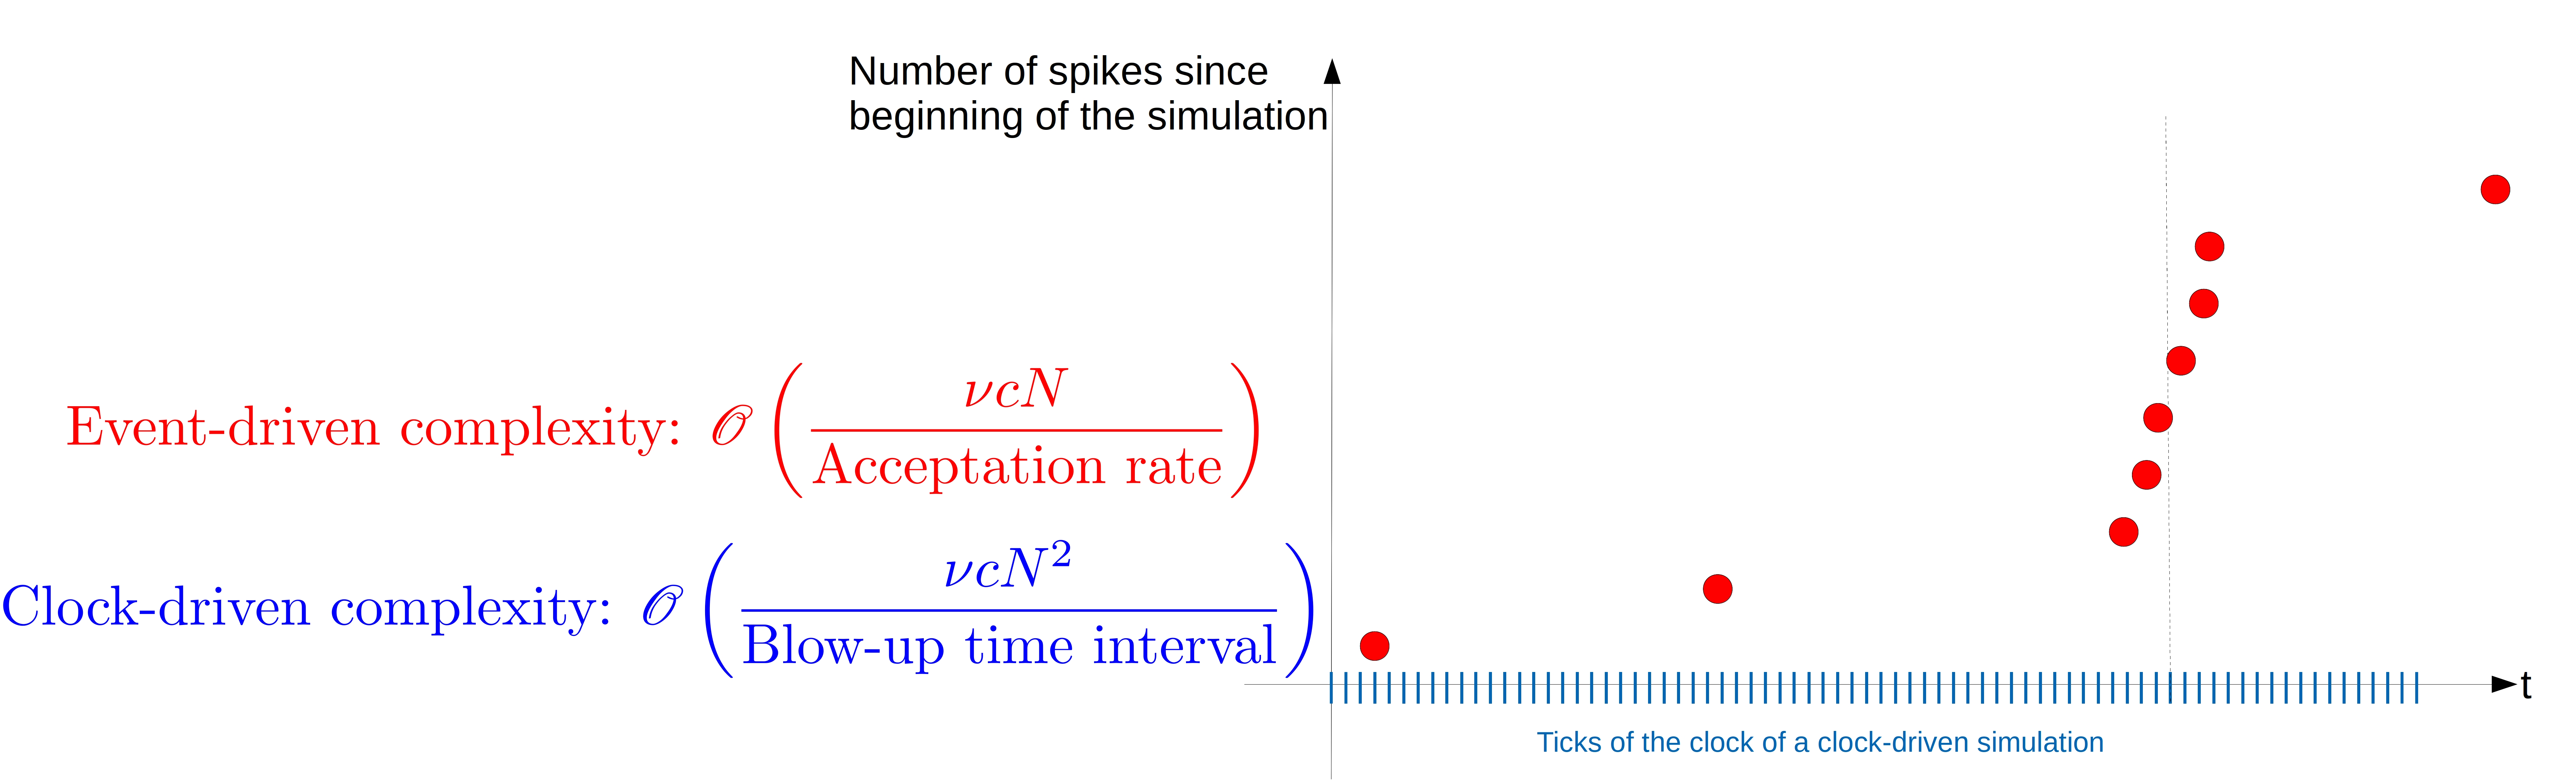
\includegraphics{complexity}
			\caption{Size of discrete time steps for clock-driven simulation compared to adaptative time steps of event-driven simulations}
		\end{subfigure}
		\caption{Complexity of event-driven vs clock-driven}
	\end{figure}
	The complexity of clock-driven algorithms is of order $N^2$. Event-driven algorithms have much less complexity, of order N. But as our algorithm is based on athinning method, the complexity is higher, but still linear of N.
\end{document}